\section{Gluon radiation from a parent gluon}
\begin{figure}[ht!]
\centering
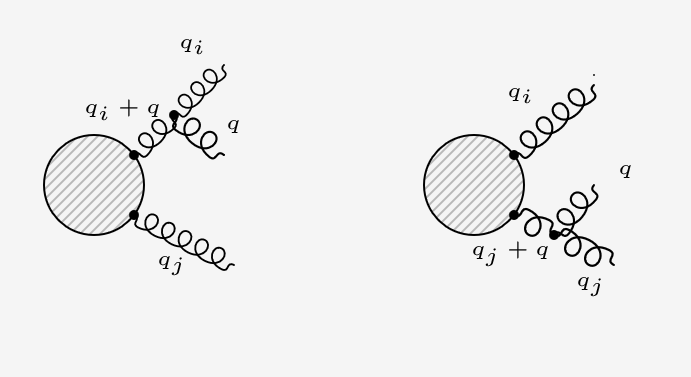
\includegraphics[width=0.85\textwidth]{images/GG/GGDiagrams.png}
\end{figure}
Now consider a daughter gluon from the splitting of a parent gluon with radiation an another gluon. When the gluon becomes soft, the distinction between daughter and parent vanishes, and a singularity develops. In this chapter we are going to keep the same procedure with a difference that we will not use the old parametrisation since it only works in LO. One of the mainly challenges about this emission kernel is that the calculations are long and complicated.

\subsection{Gluon-Emitter Bubble}
\begin{figure}[ht!]
\centering
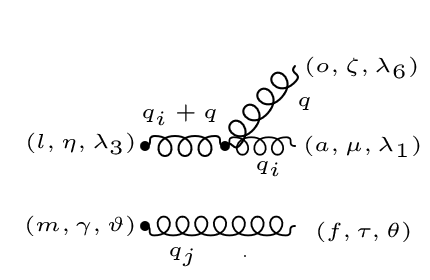
\includegraphics[scale=0.7]{images/GG/M1gg.png}
\end{figure}
Beginning with Feynman rules for this diagram as usual:
%\begin{equation}
%\begin{split}
%M_1=[\frac{-i}{(q +q_i)^2}(-g_s f^{\:a\:o\:l}(g^{{\mu}{\zeta}}(q -q_i)^{\eta}+g^{{\zeta}{\eta}}(-q-(q +q_i))^{\mu}+g^{{\eta}{\mu}}(q_i +q_i+q)^{\zeta})\\
%{\varepsilon^{\lambda_1}}_{\mu} (q) {\varepsilon^{\lambda_6}}_{\zeta} (q)][{{\varepsilon^{\theta}}_{{\tau}^{\prime}}} (q_j)]
%\end{split}
%\end{equation}
\begin{equation}
\begin{split}
M_1=&[\frac{-i}{(q_i +q)^2}(-g_s f^{\:a\:o\:l}(g^{{\mu}{\zeta}}(q-q_i)^{\eta}-g^{{\zeta}{\eta}}(2q +q_i)^{\mu}+g^{{\eta}{\mu}}(2q_i +q)^{\zeta})\\
&{\varepsilon^{\lambda_1}}_{\mu} (q_i) {\varepsilon^{\lambda_6}}_{\zeta} (q)][{{\varepsilon^{\theta}}_{{\tau}^{\prime}}} (q_j)]
\end{split}
\end{equation}
It has to be emphasized that here only the momentum from the parent gluon is incoming and the two further momenta from the vertex are outgoing. This is why the minus signs appear in the equation.
If the upper equation is daggered the following diagram will be catch and the corresponding following amplitude:

\begin{figure}[ht!]
\centering
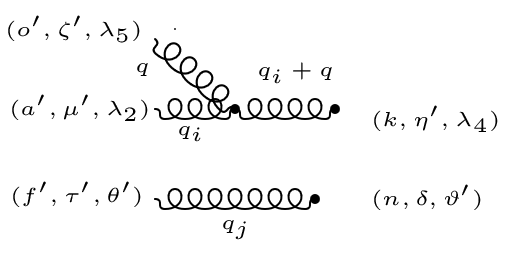
\includegraphics[scale=0.7]{images/GG/M1Daggergg.png}
\end{figure}

\begin{equation}
\begin{split}
{M_1}^{\dagger}=&[\frac{i}{(q_i +q)^2}(-g_s f^{\:a^{\prime}\:k\: o^{\prime}}(-g^{{{\mu}^{\prime}}{{\eta}^{\prime}}}(2q_i+q)^{{\zeta}^{\prime}}+g^{{{\eta}^{\prime}}{{\zeta}^{\prime}}}(2q +q_i)^{{\mu}^{\prime}}+g^{{{\zeta}^{\prime}}{{\mu}^{\prime}}}(q_i-q)^{{\eta}^{\prime}})\\
&{{\varepsilon^{\lambda_2}}_{{\mu}^{\prime}}}^* (q_i) {{\varepsilon^{\lambda_5}}_{{\zeta}^{\prime}}}^* (q)][{{\varepsilon^{{\theta}^{\prime}}}_{{\tau}^{\prime}}}^* (q_j)]
\end{split}
\end{equation}


Calculating of the matrix element:

\begin{figure}[h!]
\centering
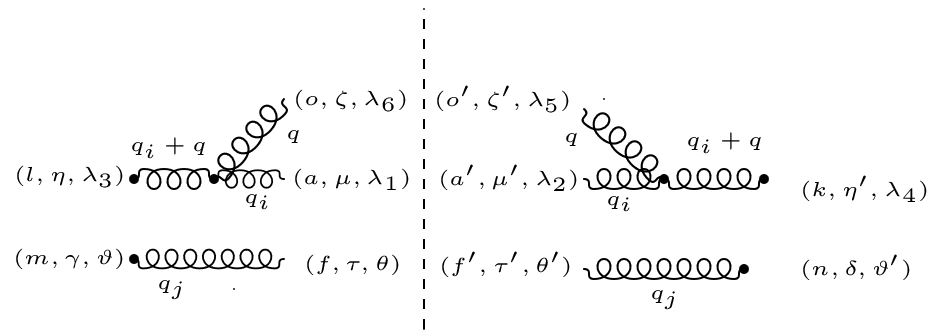
\includegraphics[width=0.95\textwidth]{images/GG/M1Squer.png}
\end{figure}
\begin{equation}
\begin{split}
|M_1|^2=&[\frac{-i}{(q_i +q)^2}(-g_s f^{\:a\:o\:l}(g^{{\mu}{\zeta}}(q-q_i)^{\eta}-g^{{\zeta}{\eta}}(2q +q_i)^{\mu}+g^{{\eta}{\mu}}(2q_i +q)^{\zeta})\\
&{\varepsilon^{\lambda_1}}_{\mu} (q_i)\:{{\varepsilon^{\lambda_2}}_{{\mu}^{\prime}}}^* (q_i) {\varepsilon^{\lambda_6}}_{\zeta} (q)\:{{\varepsilon^{\lambda_5}}_{{\zeta}^{\prime}}}^* (q)
(-g_s f^{\:a^{\prime}\:k\:o^{\prime}}(-g^{{{\mu}^{\prime}}{{\eta}^{\prime}}}(2q_i+q)^{{\zeta}^{\prime}}+g^{{{\eta}^{\prime}}{{\zeta}^{\prime}}}(2q +q_i)^{{\mu}^{\prime}}\\
&+g^{{{\zeta}^{\prime}}{{\mu}^{\prime}}}(q_i-q)^{{\eta}^{\prime}})\frac{i}{(q_i +q)^2}][g^{{\gamma}{\delta}}]
\end{split}
\end{equation}

After the summation over the spin- just as well polarization indices can be obtained:
\begin{equation}
\begin{split}
|M_1|^2=\frac{g_s^2 \:f^{\:a\:o\:l}\: f^{\:a\:k\:o}}{(q_i +q)^2 (q_i +q)^2} [N^{{\eta}{{\eta}^{\prime}}}][g^{{\gamma}{\delta}}]
\end{split}
\end{equation}

The tensor $N^{{\eta}{{\eta}^{\prime}}}$ appears exactly when all possible indices contract.\\
The goal of the next step is to evaluate this tensor, which is avoided here and instead of that, it only presents the final result. The more detailed calculation can be found in Appendix section \label{tensor}.

\begin{equation}
\begin{split}
N^{{\eta}{{\eta}^{\prime}}}\equiv &[(6-d){q}^{{\eta}}{q}^{{\eta}^{\prime}}+(d+3){q}^{{\eta}}{q_i}^{{\eta}^{\prime}}+(d+3){q_i}^{{\eta}}{q}^{{\eta}^{\prime}}+(6-d){q_i}^{{\eta}}{q_i}^{{\eta}^{\prime}}\\
&-g^{{\eta}{{\eta}^{\prime}}}(5{q}^2+5{q_i}^2+8qq_i)][g^{{\gamma}{\delta}}]
\end{split}
\end{equation}
Replacing this result in the equation:
\begin{equation}
\begin{split}
|M_1|^2=&\frac{g_s^2 \:f^{\:a\:o\:l}\: f^{\:a\:k\:o}}{(q_i +q)^2 (q_i +q)^2} [(6-d){q}^{{\eta}}{q}^{{\eta}^{\prime}}+(d+3){q}^{{\eta}}{q_i}^{{\eta}^{\prime}}+(d+3){q_i}^{{\eta}}{q}^{{\eta}^{\prime}}+(6-d){q_i}^{{\eta}}{q_i}^{{\eta}^{\prime}}\\
&-g^{{\eta}{{\eta}^{\prime}}}(5{q}^2+5{q_i}^2+8qq_i)][g^{{\gamma}{\delta}}]
\end{split}
\end{equation}

This Gluon self-energy diagram has to be corrected by ghost Loop to get the complete result. 

\pagebreak
\subsubsection{One-loop corrections to the gluon self-energy diagram(Gluon-Emitter Bubble)}
\begin{figure}[h!]
\centering
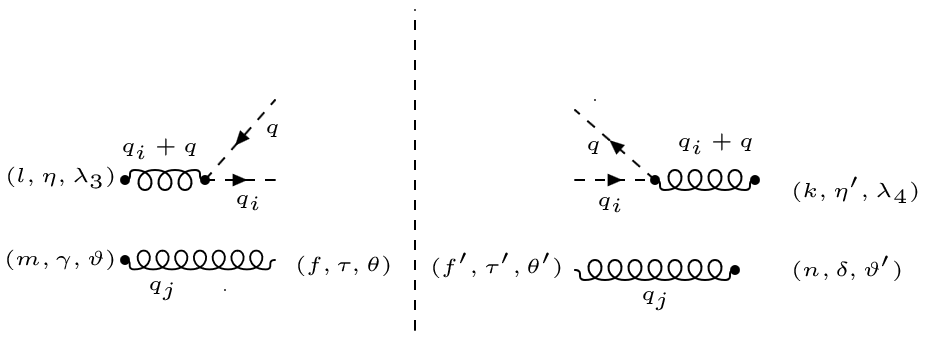
\includegraphics[width=0.95\textwidth]{images/GG/Ghost.png}
\end{figure}
In order to get a meaningful result and correct the gluon loop, the same indices must be used. For this the same diagram with a fine difference is used, in which the cut off gluon propagators is replaced with ghost propagators and the rest remain as in the previous diagram.
\begin{equation}
\begin{split}
{{|M_1|}^2_{Ghost \:loop}}=\frac{g_s^2 \:f^{\:a\:o\:l}\: f^{\:a\:k\:o}}{(q_i +q)^2 (q_i +q)^2} [-{q_i}^{{\eta}}{q}^{{\eta}^{\prime}}-{q}^{{\eta}}{q_i}^{{\eta}^{\prime}}][g^{{\gamma}{\delta}}]
\end{split}
\end{equation}

\begin{equation}
\begin{split}
&{|{M}^{\prime}_1|}^2 = {|M_1|}^2+{{|M_1|}^2_{Ghost \:loop}}=\frac{g_s^2 \:f^{\:a\:o\:l}\: f^{\:a\:k\:o}}{(q_i +q)^2 (q_i +q)^2}  [(6-d){q}^{{\eta}}{q}^{{\eta}^{\prime}}+(d+3){q}^{{\eta}}{q_i}^{{\eta}^{\prime}}\\
&+(d+3){q_i}^{{\eta}}{q}^{{\eta}^{\prime}}+(6-d){q_i}^{{\eta}}{q_i}^{{\eta}^{\prime}}-g^{{\eta}{{\eta}^{\prime}}}(5{q}^2+5{q_i}^2+8qq_i)-{q_i}^{{\eta}}{q}^{{\eta}^{\prime}}-{q}^{{\eta}}{q_i}^{{\eta}^{\prime}}][g^{{\gamma}{\delta}}]
\end{split}
\end{equation}
After simplification and addition over the same terms:
\begin{equation}
\begin{split}
&{|{M}^{\prime}_1|}^2 =\frac{g_s^2 \:f^{\:a\:o\:l}\: f^{\:a\:k\:o}}{(q_i +q)^2 (q_i +q)^2}  [(6-d){q}^{{\eta}}{q}^{{\eta}^{\prime}}+(d+2){q}^{{\eta}}{q_i}^{{\eta}^{\prime}}+(d+2){q_i}^{{\eta}}{q}^{{\eta}^{\prime}}+(6-d){q_i}^{{\eta}}{q_i}^{{\eta}^{\prime}}\\
&-g^{{\eta}{{\eta}^{\prime}}}(8qq_i)][g^{{\gamma}{\delta}}]
\end{split}
\end{equation}

Implementation the new parametrisation:

\begin{equation}
\begin{split}
&{|{M}^{\prime}_1|}^2 =\frac{g_s^2 \:f^{\:a\:o\:l}\: f^{\:a\:k\:o}}{4y^2({\alpha_1}+\beta_1)^2\:(p_i\cdot Q) \:(p_i\cdot Q)} \\
&[(6-d)(\zeta_1 {p_i}^{\eta} + \lambda_1{Q}^{\eta} + \sqrt{y\alpha_1\beta_1}{n^{\eta}}_{\bot,1})(\zeta_1 {p_i}^{{\eta}^{\prime}} + \lambda_1{Q}^{{\eta}^{\prime}} + \sqrt{y\alpha_1\beta_1}{n^{{\eta}^{\prime}}}_{\bot,1})\\
&+(d+2)(\zeta_1 {p_i}^{\eta} + \lambda_1{Q}^{\eta} + \sqrt{y\alpha_1\beta_1}{n^{\eta}}_{\bot,1})(\zeta_q {p_i}^{{\eta}^{\prime}} + \lambda_q{Q}^{{\eta}^{\prime}} - \sqrt{y\alpha_1\beta_1}{n^{{\eta}^{\prime}}}_{\bot,1})\\
&+(d+2)(\zeta_q {p_i}^{\eta} + \lambda_q{Q}^{\eta} - \sqrt{y\alpha_1\beta_1}{n^{\eta}}_{\bot,1})(\zeta_1 {p_i}^{{\eta}^{\prime}} + \lambda_1{Q}^{{\eta}^{\prime}} + \sqrt{y\alpha_1\beta_1}{n^{{\eta}^{\prime}}}_{\bot,1})\\
&+(6-d)(\zeta_q {p_i}^{\eta} + \lambda_q{Q}^{\eta} - \sqrt{y\alpha_1\beta_1}{n^{\eta}}_{\bot,1})(\zeta_q {p_i}^{{\eta}^{\prime}} + \lambda_q{Q}^{{\eta}^{\prime}} - \sqrt{y\alpha_1\beta_1}{n^{{\eta}^{\prime}}}_{\bot,1})\\
&-8g^{{\eta}{{\eta}^{\prime}}}[({\alpha_1}^2+{\beta_1}^2) p_i \cdot Q - ({\beta_1}(1-\beta_1)){n}_{\bot,1}\cdot{n}_{\bot,1}]][g^{{\gamma}{{\delta}}}]
\end{split}
\end{equation}

Note that here the short version of the kinematics was used to increase the overview. Now the terms in brackets have to be multiplied and simplified.

\begin{equation}
\begin{split}
&{|{M}^{\prime}_1|}^2 =\frac{g_s^2 \:f^{\:a\:o\:l}\: f^{\:a\:k\:o}}{y^2\:(p_i\cdot Q) \:(p_i\cdot Q)} 
[(6-d)[\zeta_1 \zeta_1 {p_i}^{\eta}{p_i}^{{\eta}^{\prime}}+\zeta_1 \lambda_1{p_i}^{\eta}{Q}^{{\eta}^{\prime}}+\zeta_1\sqrt{y\alpha_1\beta_1}{p_i}^{\eta}{n^{{\eta}^{\prime}}}_{\bot,1}\\
&+\lambda_1\zeta_1 {Q}^{\eta}{p_i}^{{\eta}^{\prime}}+\lambda_1\lambda_1{Q}^{\eta}{Q}^{{\eta}^{\prime}}+\lambda_1\sqrt{y\alpha_1\beta_1}{Q}^{\eta}{n^{{\eta}^{\prime}}}_{\bot,1}
+\zeta_1\sqrt{y\alpha_1\beta_1} {n^{{\eta}}}_{\bot,1}{p_i}^{{\eta}^{\prime}}+\lambda_1\sqrt{y\alpha_1\beta_1}{n^{{\eta}}}_{\bot,1}{Q}^{{\eta}^{\prime}}\\
&+\sqrt{y\alpha_1\beta_1}\sqrt{y\alpha_1\beta_1}{n^{{\eta}}}_{\bot,1}{n^{{\eta}^{\prime}}}_{\bot,1}]
[(d+2)[\zeta_1 \zeta_q {p_i}^{\eta}{p_i}^{{\eta}^{\prime}}+\zeta_1 \lambda_q{p_i}^{\eta}{Q}^{{\eta}^{\prime}}-\zeta_1\sqrt{y\alpha_1\beta_1}{p_i}^{\eta}{n^{{\eta}^{\prime}}}_{\bot,1}\\
&+\lambda_1\zeta_q {Q}^{\eta}{p_i}^{{\eta}^{\prime}}+\lambda_1\lambda_q{Q}^{\eta}{Q}^{{\eta}^{\prime}}-\lambda_1\sqrt{y\alpha_1\beta_1}{Q}^{\eta}{n^{{\eta}^{\prime}}}_{\bot,1}+\zeta_q\sqrt{y\alpha_1\beta_1} {n^{{\eta}}}_{\bot,1}{p_i}^{{\eta}^{\prime}}+\lambda_q\sqrt{y\alpha_1\beta_1}{n^{{\eta}}}_{\bot,1}{Q}^{{\eta}^{\prime}}\\
&-\sqrt{y\alpha_1\beta_1}\sqrt{y\alpha_1\beta_1}{n^{{\eta}}}_{\bot,1}{n^{{\eta}^{\prime}}}_{\bot,1}][(d+2)[\zeta_q \zeta_1 {p_i}^{\eta}{p_i}^{{\eta}^{\prime}}+\zeta_q \lambda_1{p_i}^{\eta}{Q}^{{\eta}^{\prime}}+\zeta_q\sqrt{y\alpha_1\beta_1}{p_i}^{\eta}{n^{{\eta}^{\prime}}}_{\bot,1}\\
&+\lambda_q\zeta_1 {Q}^{\eta}{p_i}^{{\eta}^{\prime}}+\lambda_q\lambda_1{Q}^{\eta}{Q}^{{\eta}^{\prime}}+\lambda_q\sqrt{y\alpha_1\beta_1}{Q}^{\eta}{n^{{\eta}^{\prime}}}_{\bot,1}-\zeta_1\sqrt{y\alpha_1\beta_1} {n^{{\eta}}}_{\bot,1}{p_i}^{{\eta}^{\prime}}-\lambda_1\sqrt{y\alpha_1\beta_1}{n^{{\eta}}}_{\bot,1}{Q}^{{\eta}^{\prime}}\\
&-\sqrt{y\alpha_1\beta_1}\sqrt{y\alpha_1\beta_1}{n^{{\eta}}}_{\bot,1}{n^{{\eta}^{\prime}}}_{\bot,1}][(6-d)[\zeta_q \zeta_q {p_i}^{\eta}{p_i}^{{\eta}^{\prime}}+\zeta_q \lambda_q{p_i}^{\eta}{Q}^{{\eta}^{\prime}}-\zeta_q\sqrt{y\alpha_1\beta_1}{p_i}^{\eta}{n^{{\eta}^{\prime}}}_{\bot,1}\\
&+\lambda_q\zeta_q {Q}^{\eta}{p_i}^{{\eta}^{\prime}}+\lambda_q\lambda_q{Q}^{\eta}{Q}^{{\eta}^{\prime}}-\lambda_q\sqrt{y\alpha_1\beta_1}{Q}^{\eta}{n^{{\eta}^{\prime}}}_{\bot,1}-\zeta_q\sqrt{y\alpha_1\beta_1} {n^{{\eta}}}_{\bot,1}{p_i}^{{\eta}^{\prime}}-\lambda_q\sqrt{y\alpha_1\beta_1}{n^{{\eta}}}_{\bot,1}{Q}^{{\eta}^{\prime}}\\
&+\sqrt{y\alpha_1\beta_1}\sqrt{y\alpha_1\beta_1}{n^{{\eta}}}_{\bot,1}{n^{{\eta}^{\prime}}}_{\bot,1}-8g^{{\eta}{{\eta}^{\prime}}}[({\alpha_1}^2+{\beta_1}^2) p_i \cdot Q - ({\beta_1}(1-\beta_1)){n}_{\bot,1}\cdot{n}_{\bot,1}]][g^{{\gamma}{{\delta}}}]
\end{split}
\end{equation}


One replaces now the relations for the often occurring pre-factor products from appendix \ref{pre}:
%\begin{equation}
%\begin{split}
%{|{M}^{\prime}_1|}^2 =\frac{g_s^2 \:f^{\:a\:o\:l}\: f^{\:a\:k\:o}}{4y^2\:(p_i\cdot Q) \:(p_i\cdot Q)} \\
%[(6-d)[({\alpha_1}^2 -2y\alpha_1 \beta_1(\frac{Q^2}{2p_i \cdot Q})+y^2{\beta_1}^2(\frac{Q^2}{2p_i \cdot Q})^2) {p_i}^{\eta}{p_i}^{{\eta}^{\prime}}\\+(y\alpha_1\beta_1 -{y^2\beta_1}^2(\frac{Q^2}{2p_i \cdot Q})){p_i}^{\eta}{Q}^{{\eta}^{\prime}}+\zeta_1\sqrt{y\alpha_1\beta_1}{p_i}^{\eta}{n^{{\eta}^{\prime}}}_{\bot,1}\\
%+(y\beta_1\alpha_1 -y^2{\beta_1}^2(\frac{Q^2}{2p_i \cdot Q})) {Q}^{\eta}{p_i}^{{\eta}^{\prime}}+y^2{\beta_1}^2{Q}^{\eta}{Q}^{{\eta}^{\prime}}+\lambda_1\sqrt{y\alpha_1\beta_1}{Q}^{\eta}{n^{{\eta}^{\prime}}}_{\bot,1}\\
%+\zeta_1\sqrt{y\alpha_1\beta_1} {n^{{\eta}}}_{\bot,1}{p_i}^{{\eta}^{\prime}}+\lambda_1\sqrt{y\alpha_1\beta_1}{n^{{\eta}}}_{\bot,1}{Q}^{{\eta}^{\prime}}+\sqrt{y\alpha_1\beta_1}\sqrt{y\alpha_1\beta_1}{n^{{\eta}}}_{\bot,1}{n^{{\eta}^{\prime}}}_{\bot,1}]\\
%[(d+2)[(\alpha_1\beta_1-y({\alpha_1}^2+{\beta_1}^2) (\frac{Q^2}{2p_i \cdot Q})+y^2{\alpha_1}{\beta_1}(\frac{Q^2}{2p_i \cdot Q})^2) {p_i}^{\eta}{p_i}^{{\eta}^{\prime}}\\+(y{\alpha_1}^2 -y^2\beta_1\alpha_1(\frac{Q^2}{2p_i \cdot Q})){p_i}^{\eta}{Q}^{{\eta}^{\prime}}-\zeta_1\sqrt{y\alpha_1\beta_1}{p_i}^{\eta}{n^{{\eta}^{\prime}}}_{\bot,1}\\
%+(y{\beta_1}^2 -y^2\alpha_1 \beta_1(\frac{Q^2}{2p_i \cdot Q})) {Q}^{\eta}{p_i}^{{\eta}^{\prime}}+y^2\beta_1\alpha_1{Q}^{\eta}{Q}^{{\eta}^{\prime}}\\-\lambda_1\sqrt{y\alpha_1\beta_1}{Q}^{\eta}{n^{{\eta}^{\prime}}}_{\bot,1}
%+\zeta_q\sqrt{y\alpha_1\beta_1} {n^{{\eta}}}_{\bot,1}{p_i}^{{\eta}^{\prime}}\\+\lambda_q\sqrt{y\alpha_1\beta_1}{n^{{\eta}}}_{\bot,1}{Q}^{{\eta}^{\prime}}-\sqrt{y\alpha_1\beta_1}\sqrt{y\alpha_1\beta_1}{n^{{\eta}}}_{\bot,1}{n^{{\eta}^{\prime}}}_{\bot,1}]\\
%[(d+2)[(\beta_1\alpha_1-y({\beta_1}^2+{\alpha_1}^2)(\frac{Q^2}{2p_i \cdot Q})+y^2\alpha_1\beta_1 (\frac{Q^2}{2p_i \cdot Q})^2) {p_i}^{\eta}{p_i}^{{\eta}^{\prime}}\\+(y{\beta_1}^2 -y^2\alpha_1 \beta_1(\frac{Q^2}{2p_i \cdot Q})){p_i}^{\eta}{Q}^{{\eta}^{\prime}}+\zeta_q\sqrt{y\alpha_1\beta_1}{p_i}^{\eta}{n^{{\eta}^{\prime}}}_{\bot,1}\\
%+(y{\alpha_1}^2 -y^2\alpha_1\beta_1(\frac{Q^2}{2p_i \cdot Q})) {Q}^{\eta}{p_i}^{{\eta}^{\prime}}+y^2\alpha_1\beta_1{Q}^{\eta}{Q}^{{\eta}^{\prime}}\\+\lambda_q\sqrt{y\alpha_1\beta_1}{Q}^{\eta}{n^{{\eta}^{\prime}}}_{\bot,1}\\
%-\zeta_1\sqrt{y\alpha_1\beta_1} {n^{{\eta}}}_{\bot,1}{p_i}^{{\eta}^{\prime}}-\lambda_1\sqrt{y\alpha_1\beta_1}{n^{{\eta}}}_{\bot,1}{Q}^{{\eta}^{\prime}}-\sqrt{y\alpha_1\beta_1}\sqrt{y\alpha_1\beta_1}{n^{{\eta}}}_{\bot,1}{n^{{\eta}^{\prime}}}_{\bot,1}]\\
%[(6-d)[({\beta_1}^2 -2y\alpha_1\beta_1 (\frac{Q^2}{2p_i \cdot Q})+ y^2{\alpha_1}^2 (\frac{Q^2}{2p_i \cdot Q})^2) {p_i}^{\eta}{p_i}^{{\eta}^{\prime}}\\+(y\beta_1\alpha_1 -y^2{\alpha_1}^2(\frac{Q^2}{2p_i \cdot Q})){p_i}^{\eta}{Q}^{{\eta}^{\prime}}-\zeta_q\sqrt{y\alpha_1\beta_1}{p_i}^{\eta}{n^{{\eta}^{\prime}}}_{\bot,1}\\
%+(y\alpha_1\beta_1 -y^2{\alpha_1}^2 (\frac{Q^2}{2p_i \cdot Q})) {Q}^{\eta}{p_i}^{{\eta}^{\prime}}+y^2{\alpha_1}^2{Q}^{\eta}{Q}^{{\eta}^{\prime}}-\lambda_q\sqrt{y\alpha_1\beta_1}{Q}^{\eta}{n^{{\eta}^{\prime}}}_{\bot,1}\\
%-\zeta_q\sqrt{y\alpha_1\beta_1} {n^{{\eta}}}_{\bot,1}{p_i}^{{\eta}^{\prime}}-\lambda_q\sqrt{y\alpha_1\beta_1}{n^{{\eta}}}_{\bot,1}{Q}^{{\eta}^{\prime}}\\+\sqrt{y\alpha_1\beta_1}\sqrt{y\alpha_1\beta_1}{n^{{\eta}}}_{\bot,1}{n^{{\eta}^{\prime}}}_{\bot,1}-8g^{{\eta}{{\eta}^{\prime}}}[({\alpha_1}^2+{\beta_1}^2) p_i \cdot Q - ({\beta_1}(1-\beta_1)){n}_{\bot,1}\cdot{n}_{\bot,1}]][g^{{\gamma}{{\delta}}}]
%\end{split}
%\end{equation}


%\begin{equation}
%\begin{split}
%&{|{M}^{\prime}_1|}^2 =\frac{g_s^2 \:f^{\:a\:o\:l}\: f^{\:a\:k\:o}}{4y^2\:(p_i\cdot Q) \:(p_i\cdot Q)}[(6-d)\lbrace({\alpha_1}^2 -2y\alpha_1 \beta_1(\frac{Q^2}{2p_i \cdot Q})) {p_i}^{\eta}{p_i}^{{\eta}^{\prime}}+y\alpha_1\beta_1 {p_i}^{\eta}{Q}^{{\eta}^{\prime}}\\
%&+\zeta_1\sqrt{y\alpha_1\beta_1}{p_i}^{\eta}{n^{{\eta}^{\prime}}}_{\bot,1}+y\beta_1\alpha_1  {Q}^{\eta}{p_i}^{{\eta}^{\prime}}+\lambda_1\sqrt{y\alpha_1\beta_1}{Q}^{\eta}{n^{{\eta}^{\prime}}}_{\bot,1}
%+\zeta_1\sqrt{y\alpha_1\beta_1} {n^{{\eta}}}_{\bot,1}{p_i}^{{\eta}^{\prime}}\\
%&+\lambda_1\sqrt{y\alpha_1\beta_1}{n^{{\eta}}}_{\bot,1}{Q}^{{\eta}^{\prime}}+y\alpha_1\beta_1{n^{{\eta}}}_{\bot,1}{n^{{\eta}^{\prime}}}_{\bot,1}\rbrace
%+(d+2)\lbrace(\alpha_1\beta_1-y({\alpha_1}^2+{\beta_1}^2) (\frac{Q^2}{2p_i \cdot Q})) {p_i}^{\eta}{p_i}^{{\eta}^{\prime}}\\
%&+y{\alpha_1}^2{p_i}^{\eta}{Q}^{{\eta}^{\prime}}-\zeta_1\sqrt{y\alpha_1\beta_1}{p_i}^{\eta}{n^{{\eta}^{\prime}}}_{\bot,1}+y{\beta_1}^2 {Q}^{\eta}{p_i}^{{\eta}^{\prime}}-\lambda_1\sqrt{y\alpha_1\beta_1}{Q}^{\eta}{n^{{\eta}^{\prime}}}_{\bot,1}
%+\zeta_q\sqrt{y\alpha_1\beta_1} {n^{{\eta}}}_{\bot,1}{p_i}^{{\eta}^{\prime}}\\
%&+\lambda_q\sqrt{y\alpha_1\beta_1}{n^{{\eta}}}_{\bot,1}{Q}^{{\eta}^{\prime}}-y\alpha_1\beta_1{n^{{\eta}}}_{\bot,1}{n^{{\eta}^{\prime}}}_{\bot,1}\rbrace+(d+2)\lbrace(\beta_1\alpha_1-y({\beta_1}^2+{\alpha_1}^2)(\frac{Q^2}{2p_i \cdot Q})) {p_i}^{\eta}{p_i}^{{\eta}^{\prime}}\\
%&+y{\beta_1}^2{p_i}^{\eta}{Q}^{{\eta}^{\prime}}+\zeta_q\sqrt{y\alpha_1\beta_1}{p_i}^{\eta}{n^{{\eta}^{\prime}}}_{\bot,1}+y{\alpha_1}^2 {Q}^{\eta}{p_i}^{{\eta}^{\prime}}+\lambda_q\sqrt{y\alpha_1\beta_1}{Q}^{\eta}{n^{{\eta}^{\prime}}}_{\bot,1}-\zeta_1\sqrt{y\alpha_1\beta_1} {n^{{\eta}}}_{\bot,1}{p_i}^{{\eta}^{\prime}}-\lambda_1\sqrt{y\alpha_1\beta_1}{n^{{\eta}}}_{\bot,1}{Q}^{{\eta}^{\prime}}\\
%&-y\alpha_1\beta_1{n^{{\eta}}}_{\bot,1}{n^{{\eta}^{\prime}}}_{\bot,1}\rbrace
%+(6-d)\lbrace({\beta_1}^2 -2y\alpha_1\beta_1 (\frac{Q^2}{2p_i \cdot Q})) {p_i}^{\eta}{p_i}^{{\eta}^{\prime}}+y\beta_1\alpha_1 {p_i}^{\eta}{Q}^{{\eta}^{\prime}}\\
%&-\zeta_q\sqrt{y\alpha_1\beta_1}{p_i}^{\eta}{n^{{\eta}^{\prime}}}_{\bot,1}
%+y\alpha_1\beta_1 {Q}^{\eta}{p_i}^{{\eta}^{\prime}}-\lambda_q\sqrt{y\alpha_1\beta_1}{Q}^{\eta}{n^{{\eta}^{\prime}}}_{\bot,1}-\zeta_q\sqrt{y\alpha_1\beta_1} {n^{{\eta}}}_{\bot,1}{p_i}^{{\eta}^{\prime}}\\
%&-\lambda_q\sqrt{y\alpha_1\beta_1}{n^{{\eta}}}_{\bot,1}{Q}^{{\eta}^{\prime}}+y\alpha_1\beta_1{n^{{\eta}}}_{\bot,1}{n^{{\eta}^{\prime}}}_{\bot,1}\rbrace-8g^{{\eta}{{\eta}^{\prime}}}[({\alpha_1}^2+{\beta_1}^2) p_i \cdot Q - ({\beta_1}(1-\beta_1)){n}_{\bot,1}\cdot{n}_{\bot,1}]\\
%&[g^{{\gamma}{{\delta}}}]
%\end{split}
%\end{equation}


\begin{equation}
\begin{split}
&{|{M}^{\prime}_1|}^2 =\frac{g_s^2 \:f^{\:a\:o\:l}\: f^{\:a\:k\:o}}{4y^2\:(p_i\cdot Q) \:(p_i\cdot Q)}[(6-d)\lbrace({\alpha_1}^2 -2y\alpha_1 \beta_1(\frac{Q^2}{2p_i \cdot Q})) {p_i}^{\eta}{p_i}^{{\eta}^{\prime}}\\
&+y\alpha_1\beta_1 {p_i}^{\eta}{Q}^{{\eta}^{\prime}}+y\beta_1\alpha_1  {Q}^{\eta}{p_i}^{{\eta}^{\prime}}+y\alpha_1\beta_1{n^{{\eta}}}_{\bot,1}{n^{{\eta}^{\prime}}}_{\bot,1}\rbrace\\
&+(d+2)\lbrace(\alpha_1\beta_1-y({\alpha_1}^2+{\beta_1}^2) (\frac{Q^2}{2p_i \cdot Q})) {p_i}^{\eta}{p_i}^{{\eta}^{\prime}}+y{\alpha_1}^2{p_i}^{\eta}{Q}^{{\eta}^{\prime}}+y{\beta_1}^2 {Q}^{\eta}{p_i}^{{\eta}^{\prime}}\\
&-y\alpha_1\beta_1{n^{{\eta}}}_{\bot,1}{n^{{\eta}^{\prime}}}_{\bot,1}\rbrace+(d+2)\lbrace(\beta_1\alpha_1-y({\beta_1}^2+{\alpha_1}^2)(\frac{Q^2}{2p_i \cdot Q})) {p_i}^{\eta}{p_i}^{{\eta}^{\prime}}\\
&+y{\beta_1}^2{p_i}^{\eta}{Q}^{{\eta}^{\prime}}+y{\alpha_1}^2 {Q}^{\eta}{p_i}^{{\eta}^{\prime}}-y\alpha_1\beta_1{n^{{\eta}}}_{\bot,1}{n^{{\eta}^{\prime}}}_{\bot,1}\rbrace\\
&+(6-d)\lbrace({\beta_1}^2 -2y\alpha_1\beta_1 (\frac{Q^2}{2p_i \cdot Q})) {p_i}^{\eta}{p_i}^{{\eta}^{\prime}}+y\beta_1\alpha_1 {p_i}^{\eta}{Q}^{{\eta}^{\prime}}+y\alpha_1\beta_1 {Q}^{\eta}{p_i}^{{\eta}^{\prime}}\\
&+y\alpha_1\beta_1{n^{{\eta}}}_{\bot,1}{n^{{\eta}^{\prime}}}_{\bot,1}\rbrace-8g^{{\eta}{{\eta}^{\prime}}}[({\alpha_1}^2+{\beta_1}^2) p_i \cdot Q - ({\beta_1}(1-\beta_1)){n}_{\bot,1}\cdot{n}_{\bot,1}][g^{{\gamma}{{\delta}}}]
\end{split}
\end{equation}


%\begin{equation}
%\begin{split}
%{|{M}^{\prime}_1|}^2 =\frac{g_s^2 \:f^{\:a\:o\:l}\: f^{\:a\:k\:o}}{4y^2\:(p_i\cdot Q) \:(p_i\cdot Q)} \\
%[(6-d)({\alpha_1}^2 -2y\alpha_1 \beta_1(\frac{Q^2}{2p_i \cdot Q}))+2(d+2)({\alpha_1}{\beta}_1 -y({\alpha_1}^2 +{\beta_1}^2)(\frac{Q^2}{2p_i \cdot Q}))\\+(6-d)({\beta_1}^2 -2y\alpha_1 \beta_1(\frac{Q^2}{2p_i \cdot Q})) ]{p_i}^{\eta}{p_i}^{{\eta}^{\prime}}\\
%+[2(6-d)y\alpha_1\beta_1+(d+2)y({\alpha_1}^2 +{\beta_1}^2)] {p_i}^{\eta}{Q}^{{\eta}^{\prime}}\\
%+[2(6-d)y\beta_1\alpha_1+(d+2)y({\alpha_1}^2 +{\beta_1}^2)]  {Q}^{\eta}{p_i}^{{\eta}^{\prime}}\\+[2(6-d)-2(d+2)]y\alpha_1\beta_1{n^{{\eta}}}_{\bot,1}{n^{{\eta}^{\prime}}}_{\bot,1}-8g^{{\eta}{{\eta}^{\prime}}}[({\alpha_1}^2+{\beta_1}^2) p_i \cdot Q - ({\beta_1}(1-\beta_1)){n}_{\bot,1}\cdot{n}_{\bot,1}][g^{{\gamma}{{\delta}}}]]
%\end{split}
%\end{equation}

%\begin{equation}
%\begin{split}
%{|{M}^{\prime}_1|}^2 =\frac{g_s^2 \:f^{\:a\:o\:l}\: f^{\:a\:k\:o}}{4y^2\:(p_i\cdot Q) \:(p_i\cdot Q)} \\
%[(6-d)({\alpha_1}^2 -2y\alpha_1 \beta_1(\frac{Q^2}{2p_i \cdot Q}))+2(d+2)({\alpha_1}{\beta}_1 -y({\alpha_1}^2 +{\beta_1}^2)(\frac{Q^2}{2p_i \cdot Q}))\\+(6-d)({\beta_1}^2 -2y\alpha_1 \beta_1(\frac{Q^2}{2p_i \cdot Q})) ]{p_i}^{\eta}{p_i}^{{\eta}^{\prime}}\\
%+y[(4d-8){\alpha_1}^2+(8-4d){\alpha}_1 +(d+2)] {p_i}^{\eta}{Q}^{{\eta}^{\prime}}\\
%+y[(4d-8){\alpha_1}^2+(8-4d){\alpha}_1 +(d+2)]  {Q}^{\eta}{p_i}^{{\eta}^{\prime}}\\+y[8-4d](\alpha_1-{\alpha_1}^2){n^{{\eta}}}_{\bot,1}{n^{{\eta}^{\prime}}}_{\bot,1}-8g^{{\eta}{{\eta}^{\prime}}}[({\alpha_1}^2+{\beta_1}^2) p_i \cdot Q - ({\beta_1}(1-\beta_1)){n}_{\bot,1}\cdot{n}_{\bot,1}][g^{{\gamma}{{\delta}}}]]
%\end{split}
%\end{equation}

\begin{equation}
\begin{split}
{|{M}^{\prime}_1|}^2 =&\frac{g_s^2 \:f^{\:a\:o\:l}\: f^{\:a\:k\:o}}{4y\:(p_i\cdot Q) \:(p_i\cdot Q)}[[8-4d]{\beta_1}(1-\beta_1){n^{{\eta}}}_{\bot,1}{n^{{\eta}^{\prime}}}_{\bot,1}-8g^{{\eta}{{\eta}^{\prime}}}[({\alpha_1}^2+{\beta_1}^2) p_i \cdot Q\\
&- ({\beta_1}(1-\beta_1)){n}_{\bot,1}\cdot{n}_{\bot,1}][g^{{\gamma}{{\delta}}}]]
\end{split}
\end{equation}

%\begin{equation}
%\begin{split}
%&{|{M}^{\prime}_1|}^2 =\frac{g_s^2 \:f^{\:a\:o\:l}\: f^{\:a\:k\:o}}{4y\:(p_i\cdot Q) \:(p_i\cdot Q)} 
%[8[\epsilon-1]{\beta_1}(1-\beta_1){n^{{\eta}}}_{\bot,1}{n^{{\eta}^{\prime}}}_{\bot,1}-8g^{{\eta}{{\eta}^{\prime}}}[({\alpha_1}^2+{\beta_1}^2) p_i \cdot Q \\
%&- ({\beta_1}(1-\beta_1))(-2p_i \cdot Q)][g^{{\gamma}{{\delta}}}]]
%\end{split}
%\end{equation}
%
%\begin{equation}
%\begin{split}
%&{|{M}^{\prime}_1|}^2 =\frac{g_s^2 \:f^{\:a\:o\:l}\: f^{\:a\:k\:o}}{4y\:(p_i\cdot Q) \:(p_i\cdot Q)} 
%[8[\epsilon-1]{\beta_1}(1-\beta_1){n^{{\eta}}}_{\bot,1}{n^{{\eta}^{\prime}}}_{\bot,1}-8g^{{\eta}{{\eta}^{\prime}}}[({\alpha_1}^2+{\beta_1}^2) p_i \cdot Q\\
%& +2{\alpha_1}{\beta_1} p_i \cdot Q)][g^{{\gamma}{{\delta}}}]]
%\end{split}
%\end{equation}
%
%\begin{equation}
%\begin{split}
%&{|{M}^{\prime}_1|}^2 =\frac{g_s^2 \:f^{\:a\:o\:l}\: f^{\:a\:k\:o}}{4y\:(p_i\cdot Q) \:(p_i\cdot Q)} 
%[8[\epsilon-1]{\beta_1}(1-\beta_1){n^{{\eta}}}_{\bot,1}{n^{{\eta}^{\prime}}}_{\bot,1}-8g^{{\eta}{{\eta}^{\prime}}}[({\alpha_1}+{\beta_1})^2 p_i \cdot Q)][g^{{\gamma}{{\delta}}}]]
%\end{split}
%\end{equation}
In this step the equation for $ d = 4-2 \epsilon $ was calculated and the value of $ ({\alpha_1}+{\beta_1})^2 p_i \cdot Q $ from equation \eqref{fistScalarProduct} was replaced. What here noticeable is at this point that one $ y $ from the denominator is abbreviated with one from the nominator. The final result looks like this:
\begin{equation}
\begin{split}
{|{M}^{\prime}_1|}^2 =\frac{g_s^2 \:f^{\:a\:o\:l}\: f^{\:a\:k\:o}}{y\:(p_i\cdot Q)}[2[\epsilon-1]{\beta_1}(1-\beta_1){n^{{\eta}}}_{\bot,1}{n^{{\eta}^{\prime}}}_{\bot,1}-2g^{{\eta}{{\eta}^{\prime}}}][g^{{\gamma}{{\delta}}}]
\end{split}
\end{equation}

\pagebreak

\subsection{A simplified way within the concept \ref{Concept} }
During the analysis of the evaluation it turned out that the particularly complicated and extensive calculation can be handled with the substitutions conceived below:\\
The numerator generally consists of the addition of several terms, which mostly consist of scalar products with two four-vectors. This is the reason why these scalar products have to be considered separately. The terms with the same pre-factor are eliminated from the nominator beforehand, since they are finite anyway.
In the last chapter, this has already been deduced with regard to the factors in the denominator. 
For illustration this is calculated once for ${|{M}^{\prime}_1|}^2$ with the denominator $ 4y^2\:(p_i\cdot Q) \:(p_i\cdot Q) $. \\
If one looks at this corrected matrix element, with the pre-factor $ y^2 $ in the denominator, it can be seen that in the nominator there are terms with $ y^2 $ by the multiplication of two four-vectors. Those can be neglected instead of calculating these, since exactly these are the finite terms. This simplifies the results of the scalar products. Under this assumption, the result looks as follows:

\begin{equation}
\begin{split}
{k_1}^{{\eta}}{k_1}^{{\eta}^{\prime}}&=({\alpha_1}^2 -2\alpha_1 \beta_1 y(\frac{Q^2}{2 p_i \cdot Q})){p_i}^{{\eta}}{p_i}^{{\eta}^{\prime}}+y\alpha_1 \beta_1 {p_i}^{{\eta}}{Q}^{{\eta}^{\prime}}+y\alpha_1 \beta_1 {Q}^{{\eta}}{p_i}^{{\eta}^{\prime}}+y\alpha_1\beta_1 {n}^{{\eta}}_{\bot,1}{n}^{{\eta}^{\prime}}_{\bot,1}\\
{k_1}^{{\eta}}{q_i}^{{\eta}^{\prime}}&=({\alpha_1}\beta_1 -y({\alpha_1}^2 + {\beta_1}^2 )(\frac{Q^2}{2 p_i \cdot Q})){p_i}^{{\eta}}{p_i}^{{\eta}^{\prime}}+y{\alpha_1}^2 {p_i}^{{\eta}}{Q}^{{\eta}^{\prime}}+y{\beta_1}^2 {Q}^{{\eta}}{p_i}^{{\eta}^{\prime}}-y\alpha_1\beta_1 {n}^{{\eta}}_{\bot,1}{n}^{{\eta}^{\prime}}_{\bot,1}\\
{q_i}^{{\eta}}{k_1}^{{\eta}^{\prime}}&=({\alpha_1}\beta_1 -y({\alpha_1}^2 + {\beta_1}^2 )(\frac{Q^2}{2 p_i \cdot Q})){p_i}^{{\eta}}{p_i}^{{\eta}^{\prime}}+y{\beta_1}^2 {p_i}^{{\eta}}{Q}^{{\eta}^{\prime}}+y{\alpha_1}^2 {Q}^{{\eta}}{p_i}^{{\eta}^{\prime}}-y\alpha_1\beta_1 {n}^{{\eta}}_{\bot,1}{n}^{{\eta}^{\prime}}_{\bot,1}\\
{q_i}^{{\eta}}{q_i}^{{\eta}^{\prime}}&=({\beta_1}^2 -2\alpha_1 \beta_1 y(\frac{Q^2}{2 p_i \cdot Q})){p_i}^{{\eta}}{p_i}^{{\eta}^{\prime}}+y\alpha_1 \beta_1 {p_i}^{{\eta}}{Q}^{{\eta}^{\prime}}+y\alpha_1 \beta_1 {Q}^{{\eta}}{p_i}^{{\eta}^{\prime}}+y\alpha_1\beta_1 {n}^{{\eta}}_{\bot,1}{n}^{{\eta}^{\prime}}_{\bot,1}
\end{split}
\end{equation}

Inserting these results into $ N $ follows:

\begin{equation}
\begin{split}
&N\equiv(6-d)({\alpha_1}^2 -2\alpha_1 \beta_1 y(\frac{Q^2}{2 p_i \cdot Q})){p_i}^{{\eta}}{p_i}^{{\eta}^{\prime}}+y\alpha_1 \beta_1 {p_i}^{{\eta}}{Q}^{{\eta}^{\prime}}+y\alpha_1 \beta_1 {Q}^{{\eta}}{p_i}^{{\eta}^{\prime}}+y\alpha_1\beta_1 {n}^{{\eta}}_{\bot,1}{n}^{{\eta}^{\prime}}_{\bot,1}\\
&+(d+2)({\alpha_1}\beta_1 -y({\alpha_1}^2 + {\beta_1}^2 )(\frac{Q^2}{2 p_i \cdot Q})){p_i}^{{\eta}}{p_i}^{{\eta}^{\prime}}+y{\alpha_1}^2 {p_i}^{{\eta}}{Q}^{{\eta}^{\prime}}+y{\beta_1}^2 {Q}^{{\eta}}{p_i}^{{\eta}^{\prime}}-y\alpha_1\beta_1 {n}^{{\eta}}_{\bot,1}{n}^{{\eta}^{\prime}}_{\bot,1}\\
&+(d+2)({\alpha_1}\beta_1 -y({\alpha_1}^2 + {\beta_1}^2 )(\frac{Q^2}{2 p_i \cdot Q})){p_i}^{{\eta}}{p_i}^{{\eta}^{\prime}}+y{\beta_1}^2 {p_i}^{{\eta}}{Q}^{{\eta}^{\prime}}+y{\alpha_1}^2 {Q}^{{\eta}}{p_i}^{{\eta}^{\prime}}-y\alpha_1\beta_1 {n}^{{\eta}}_{\bot,1}{n}^{{\eta}^{\prime}}_{\bot,1}\\
&+(6-d)({\beta_1}^2 -2\alpha_1 \beta_1 y(\frac{Q^2}{2 p_i \cdot Q})){p_i}^{{\eta}}{p_i}^{{\eta}^{\prime}}+y\alpha_1 \beta_1 {p_i}^{{\eta}}{Q}^{{\eta}^{\prime}}+y\alpha_1 \beta_1 {Q}^{{\eta}}{p_i}^{{\eta}^{\prime}}+y\alpha_1\beta_1 {n}^{{\eta}}_{\bot,1}{n}^{{\eta}^{\prime}}_{\bot,1}\\
&-8g^{{\eta}{{\eta}^{\prime}}}[({\alpha_1}^2+{\beta_1}^2) p_i \cdot Q - ({\beta_1}(1-\beta_1)){n}_{\bot,1}\cdot{n}_{\bot,1}]\\
\end{split}
\end{equation}

Summary of the equation provides:

\begin{equation}
\begin{split}
&N\equiv[(6-d)({\alpha_1}^2 -2\alpha_1 \beta_1 y(\frac{Q^2}{2 p_i \cdot Q}))+(d+2)({\alpha_1}\beta_1 -y({\alpha_1}^2 + {\beta_1}^2 )(\frac{Q^2}{2 p_i \cdot Q}))\\&+(d+2)({\alpha_1}\beta_1 -y({\alpha_1}^2 + {\beta_1}^2 )(\frac{Q^2}{2 p_i \cdot Q}))+(6-d)({\beta_1}^2 -2\alpha_1 \beta_1 y(\frac{Q^2}{2 p_i \cdot Q}))]{p_i}^{{\eta}}{p_i}^{{\eta}^{\prime}}\\
&+[(6-d)y\alpha_1 \beta_1+(d+2)y{\alpha_1}^2+(d+2)y{\beta_1}^2+(6-d)y\alpha_1 \beta_1] {p_i}^{{\eta}}{Q}^{{\eta}^{\prime}}\\
&+[(6-d)y\alpha_1 \beta_1 +(d+2)y{\beta_1}^2+(d+2)y{\alpha_1}^2+(6-d)y\alpha_1 \beta_1] {Q}^{{\eta}}{p_i}^{{\eta}^{\prime}}\\
&+[(6-d)y\alpha_1\beta_1-(d+2)y\alpha_1\beta_1-(d+2)y\alpha_1\beta_1+(6-d)y\alpha_1\beta_1] {n}^{{\eta}}_{\bot,1}{n}^{{\eta}^{\prime}}_{\bot,1}\\
&-8g^{{\eta}{{\eta}^{\prime}}}[({\alpha_1}^2+{\beta_1}^2) p_i \cdot Q - ({\beta_1}(1-\beta_1)){n}_{\bot,1}\cdot{n}_{\bot,1}]\\
\end{split}
\end{equation}

and for the matrix element:

%\begin{equation}
%\begin{split}
%&{|{M}^{\prime}_1|}^2 =\frac{g_s^2 \:f^{\:a\:o\:l}\: f^{\:a\:k\:o}}{4y\:(p_i\cdot Q)^2} 
%[(12-2d)y\alpha_1\beta_1-2(d+2)y\alpha_1\beta_1] {n}^{{\eta}}_{\bot,1}{n}^{{\eta}^{\prime}}_{\bot,1}-8yg^{{\eta}{{\eta}^{\prime}}} p_i \cdot Q][g_{{\gamma}{{\delta}}}]\\
%&\Rightarrow {|{M}^{\prime}_1|}^2 =\frac{g_s^2 \:f^{\:a\:o\:l}\: f^{\:a\:k\:o}}{4y\:(p_i\cdot Q)^2} 
%[(12-2d)\alpha_1\beta_1-2(d+2)\alpha_1\beta_1] {n}^{{\eta}}_{\bot,1}{n}^{{\eta}^{\prime}}_{\bot,1}
%-8g^{{\eta}{{\eta}^{\prime}}}({\alpha_1}^2+{\beta_1}^2) p_i \cdot Q][g_{{\gamma}{{\delta}}}]\\
%& {|{M}^{\prime}_1|}^2 =\frac{g_s^2 \:f^{\:a\:o\:l}\: f^{\:a\:k\:o}}{4y\:(p_i\cdot Q) \:(p_i\cdot Q)}\\
%&[8[\epsilon-1]{\beta_1}(1-\beta_1){n^{{\eta}}}_{\bot,1}{n^{{\eta}^{\prime}}}_{\bot,1}-8g^{{\eta}{{\eta}^{\prime}}}[({\alpha_1}^2+{\beta_1}^2) p_i \cdot Q - {\beta_1} \alpha_1(-2p_i \cdot Q)]][g_{{\gamma}{{\delta}}}]
%\end{split}
%\end{equation}


\begin{equation}
\begin{split}
{|{M}^{\prime}_1|}^2 =\frac{g_s^2 \:f^{\:a\:o\:l}\: f^{\:a\:k\:o}}{y\:(p_i\cdot Q)}[2[\epsilon-1]{\beta_1}(1-\beta_1){n^{{\eta}}}_{\bot,1}{n^{{\eta}^{\prime}}}_{\bot,1}-2g^{{\eta}{{\eta}^{\prime}}}][g^{{\gamma}{{\delta}}}]
\end{split}
\end{equation}
\\

\textbf{conclusion}
\\
This concept allows to achieve the same result in just a few steps. This can also be done for further calculations.
\pagebreak
\subsection{Gluon-Spectator Bubble}
\begin{figure}[ht!]
\centering
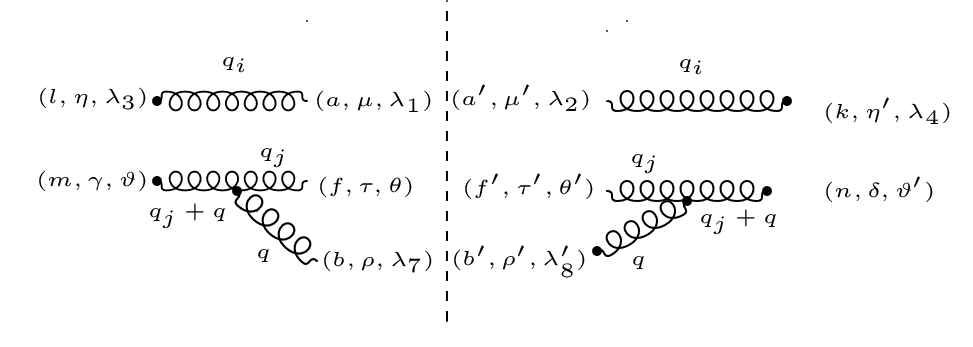
\includegraphics[width=0.95\textwidth]{images/GG/M2Squer}
\end{figure}

This concept can also be applied to the gluon spectator. The only difference is that a gluon is emitted by a spectator and other indices are used here.\\
Using the Feynmann rules, the matrix element is evaluated:

%\begin{equation}
%\begin{split}
%|M_2|^2=[\frac{-i}{(q_j +q)^2}(-g_s f^{\:b\:f\:m}(g^{{\tau}{\gamma}}(-2q_j-q)^{\rho}+g^{{\gamma}{\rho}}(2q +q_j)^{\tau}+g^{{\rho}{\tau}}(q_j -q)^{\gamma})\\g_{{\tau}{{\tau}^{\prime}}}g_{{\rho}{{\rho}^{\prime}}}
%(-g_s f^{\:b^{\prime}\:n\:f^{\prime}}(g^{{{\rho}^{\prime}}{{\delta}}}(-2q-q_j)^{{\tau}^{\prime}}+g^{{{\delta}}{{\tau}^{\prime}}}(2q_j +q)^{{\rho}^{\prime}}+g^{{{\tau}^{\prime}}{{\rho}^{\prime}}}(q-q_j)^{{\delta}})\frac{i}{(q_j +q)^2}][g^{{\eta}{{\eta}^{\prime}}}]
%\end{split}
%\end{equation}
%
%\begin{equation}
%\begin{split}
%|M_2|^2=\frac{g_s^2\: f^{\:b\:f\:m} f^{\:b^{\prime}\:n\:f^{\prime}} {\delta}^{{a}{a^{\prime}}} {\delta}^{{f}{f^{\prime}}} {\delta}^{{b}{b^{\prime}}}}{(q_j +q)^2 (q_j +q)^2}[g_{{\tau}{{\tau}^{\prime}}}g_{{\rho}{{\rho}^{\prime}}}(g^{{\tau}{\gamma}}(2q_j+q)^{\rho}g^{{{\rho}^{\prime}}{{\delta}}}(2q+q_j)^{{\tau}^{\prime}}\\
%-g^{{\tau}{\gamma}}(2q_j+q)^{\rho}g^{{{\delta}}{{\tau}^{\prime}}}(2q_j +q)^{{\rho}^{\prime}}-g^{{\tau}{\gamma}}(2q_j+q)^{\rho}g^{{{\tau}^{\prime}}{{\rho}^{\prime}}}(q-q_j)^{{\delta}}-g^{{\gamma}{\rho}}(2q +q_j)^{\tau}g^{{{\rho}^{\prime}}{{\delta}}}(2q+q_j)^{{\tau}^{\prime}}\\
%+g^{{\gamma}{\rho}}(2q +q_j)^{\tau}g^{{{\delta}}{{\tau}^{\prime}}}(2q_j +q)^{{\rho}^{\prime}}+g^{{\gamma}{\rho}}(2q +q_j)^{\tau}g^{{{\tau}^{\prime}}{{\rho}^{\prime}}}(q-q_j)^{{\delta}}-g^{{\rho}{\tau}}(q_j -q)^{\gamma}g^{{{\rho}^{\prime}}{{\delta}}}(2q+q_j)^{{\tau}^{\prime}}\\
%+g^{{\rho}{\tau}}(q_j -q)^{\gamma}g^{{{\delta}}{{\tau}^{\prime}}}(2q_j +q)^{{\rho}^{\prime}}
%+g^{{\rho}{\tau}}(q_j -q)^{\gamma}g^{{{\tau}^{\prime}}{{\rho}^{\prime}}}(q-q_j)^{{\delta}}
%][g^{{\eta}{{\eta}^{\prime}}}]
%\end{split}
%\end{equation}


\begin{equation}
\begin{split}
&|M_2|^2=\frac{g_s^2\: f^{\:b\:f\:m} f^{\:b\:n\:f}}{(q_j +q)^2 (q_j +q)^2}[(2q+q_j)^{{\gamma}}(2q_j+q)^{\delta}
-g^{{\delta}{\gamma}}(2q_j+q)^{\rho}(2q_j +q)_{{\rho}}\\&-(2q_j+q)^{\gamma}(q-q_j)^{{\delta}}-g^{{\delta}{\gamma}}(2q +q_j)^{\tau}(2q+q_j)_{{\tau}}+(2q_j +q)^{{\gamma}}(2q +q_j)^{\delta}\\
&+(2q +q_j)^{\gamma}(q-q_j)^{{\delta}}-(q_j -q)^{\gamma}(2q+q_j)^{{\delta}}+(q_j -q)^{\gamma}(2q_j +q)^{{\delta}}\\
&+d(q_j -q)^{\gamma}(q-q_j)^{{\delta}}][g^{{\eta}{{\eta}^{\prime}}}]
\end{split}
\end{equation}

It follows:

\begin{equation}
\begin{split}
&|M_2|^2=\frac{g_s^2\: f^{\:b\:f\:m} f^{\:b\:n\:f}}{(q_j +q)^2 (q_j +q)^2}[(3+d)q^{\gamma}{q_j}^{\delta}+(6-d)q^{\gamma}{q}^{\delta}+(6-d){q_j}^{\gamma}{q_j}^{\delta}\\
&+(3+d){q_j}^{\gamma}{q}^{\delta}-g^{{\delta}{\gamma}}(5{q_j}^2+5q^2+8qq_j)][g^{{\eta}{{\eta}^{\prime}}}]
\end{split}
\end{equation}





\pagebreak
\subsubsection{One-loop corrections to the gluon self-energy diagram (Gluon-Spectator Bubble)}
\begin{figure}[h!]
\centering
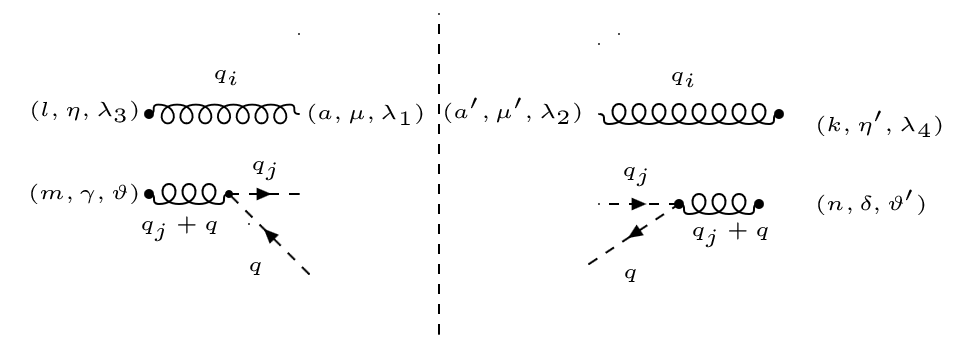
\includegraphics[width=0.95\textwidth]{images/GG/GhostM2.png}
\end{figure}
Here not all steps are shown in detail, but only the final result is presented. The reason for this is that all steps can be followed analogously to the last section.
\begin{equation}
\begin{split}
{{|M_2|}^2_{Ghost \:loop}}=\frac{g_s^2 \:f^{\:b\:f\:m} f^{\:b\:n\:f}}{(q_j +q)^2 (q_j +q)^2} [-{q_j}^{{\gamma}}{q}^{{\delta}}-{q}^{{\delta}}{q_j}^{{\gamma}}][g^{{\eta}{{\eta}^{\prime}}}]
\end{split}
\end{equation}

\begin{equation}
\begin{split}
{|{M}^{\prime}_2|}^2 =\frac{g_s^2\: f^{\:b\:f\:m} f^{\:b\:n\:f}}{(q_j +q)^2 (q_j +q)^2}[(2+d)q^{\gamma}{q_j}^{\delta}+(6-d)q^{\gamma}{q}^{\delta}\\+(6-d){q_j}^{\gamma}{q_j}^{\delta}+(2+d){q_j}^{\gamma}{q}^{\delta}-g^{{\delta}{\gamma}}(8qq_j)][g^{{\eta}{{\eta}^{\prime}}}]
\end{split}
\end{equation}
%
%\begin{equation}
%\begin{split}
%{|{M}^{\prime}_2|}^2 =\frac{g_s^2\: f^{\:b\:f\:m} f^{\:b\:n\:f}}{4(q_j \cdot q) (q_j \cdot q)}[-8g^{{\delta}{\gamma}}(q \cdot q_j)][g^{{\eta}{{\eta}^{\prime}}}]
%\end{split}
%\end{equation}
%
%\begin{equation}
%\begin{split}
%{|{M}^{\prime}_2|}^2 =\frac{g_s^2\: f^{\:b\:f\:m} f^{\:b\:n\:f}}{(q_j \cdot q)}[-2g^{{\delta}{\gamma}}][g^{{\eta}{{\eta}^{\prime}}}]
%\end{split}
%\end{equation}

\begin{equation}
\begin{split}
{|{M}^{\prime}_2|}^2 =\frac{g_s^2\: f^{\:b\:f\:m} f^{\:b\:n\:f}}{(1-\beta_1) (1-y)\:(p_i \cdot p_k)}[-2g^{{\delta}{\gamma}}][g^{{\eta}{{\eta}^{\prime}}}]
\end{split}
\end{equation}
\pagebreak

\subsection{Joining the emitter and spectator diagrams together}
\begin{figure}[h!]
\centering
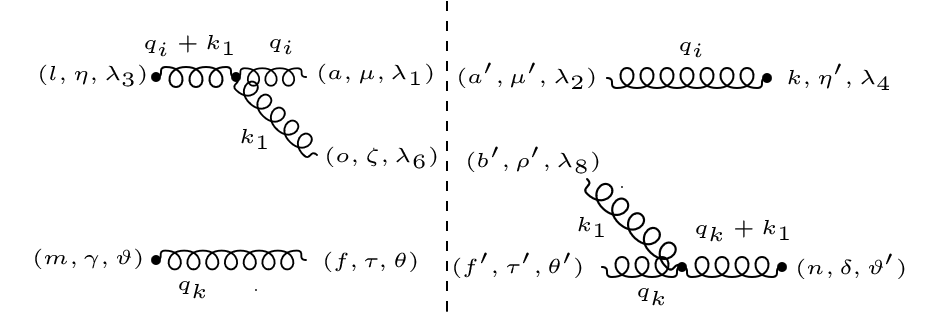
\includegraphics[width=0.95\textwidth]{images/GG/M1M2Dagger.png}
\end{figure}

Analogous to the last two sections, we calculate the quadratic matrix element in the case of the interference term.

%\begin{equation}
%\begin{split}
%&M_1{M_2}^{\dagger}=[\frac{-i}{(q_i +q)^2}(-g_s f^{\:l\:a\:o}(g^{{\eta}{\mu}}(2q_i+q)^{\zeta}+g^{{\mu}{\zeta}}(q -q_i)^{\eta}-g^{{\zeta}{\eta}}(2q +q_i)^{\mu}){\varepsilon^{\lambda_1}}_{\mu} (q_i) {\varepsilon^{\lambda_6}}_{\zeta}(q)]\\
%&[{{\varepsilon^{\theta}}_{{\tau}}}^* (q_j)]\\
%&[\frac{i}{(q +q_j)^2}(-g_s f^{\:f^{\prime}\:b^{\prime}\:n }(g^{{{\tau}^{\prime}}{{\rho}^{\prime}}}(q_j-q)^{{\delta}}+g^{{{\rho}^{\prime}}{{\delta}}}(2q +q_j)^{{\tau}^{\prime}}-g^{{{\delta}}{{\tau}^{\prime}}}(2q_j+q)^{{\rho}^{\prime}}){{\varepsilon^{{\theta}^{\prime}}}_{{\tau}^{\prime}}}^* (q_j){{\varepsilon^{\lambda_8}}_{{\rho}^{\prime}}}^* (q)]\\
%&[{{\varepsilon^{\lambda_2}}_{{\mu}^{\prime}}}^* (q_i)]
%\end{split}
%\end{equation}


\begin{equation}
\begin{split}
&M_1{M_2}^{\dagger}=\frac{g_s^2 f^{\:l\:a\:o} f^{\:f^{\prime}\: b^{\prime}\:n} \delta^{aa^{\prime}} \delta^{ob^{\prime}} \delta^{ff^{\prime}}}{(q_i +q)^2 (q_j +q)^2}
[{g_{{\mu}}}^{{\eta}^{\prime}} g_{{\tau}{{\tau}^{\prime}}}(g^{{\eta}{\mu}}(2q_i+q)^{\zeta}+g^{{\mu}{\zeta}}(q -q_i)^{\eta}-g^{{\zeta}{\eta}}(2q +q_i)^{\mu})\\
&g_{{{\zeta}}{{\rho}^{\prime}}}(g^{{{\tau}^{\prime}}{{\rho}^{\prime}}}(q_j-q)^{{\delta}}+g^{{{\rho}^{\prime}}{{\delta}}}(2q +q_j)^{{\tau}^{\prime}}-g^{{{\delta}}{{\tau}^{\prime}}}(2q_j+q)^{{\rho}^{\prime}}]
\end{split}
\end{equation}

Multiply the available tensors and summarize all results:
%\begin{equation}
%\begin{split}
%&M_1{M_2}^{\dagger}=\frac{g_s^2 f^{\:l\:a\:o} f^{\:f^{\prime}\: b^{\prime}\:n} \delta^{aa^{\prime}} \delta^{ob^{\prime}}\delta^{ff^{\prime}}}{(q_i +q)^2 (q_j +q)^2}\\
%&[g^{{{\eta}}{{\eta}^{\prime}}}(2q_i+q)^{\gamma}(q_j-q)^{{\delta}}+g^{{{\eta}}{{\eta}^{\prime}}}(2q +q_j)^{\gamma}(2q_i+q)^{{\delta}}-g^{{{\eta}}{{\eta}^{\prime}}}g^{{{\gamma}}{{\delta}}}(2q_i+q)\cdot (2q_j+q)\\
%&+g^{{{\gamma}}{{\eta}^{\prime}}}(q -q_i)^{\eta}(q_j-q)^{{\delta}}+g^{{{\eta}^{\prime}}{{\delta}}}(q -q_i)^{\eta}(2q +q_j)^{{\gamma}}
%-g^{{{\gamma}}{{\delta}}}(q -q_i)^{\eta}(2q_j+q)^{{\eta}^{\prime}}\\
%&-g^{{{\gamma}}{{\eta}}}(2q +q_i)^{{\eta}^{\prime}}(q_j-q)^{{\delta}}
%-g^{{{\eta}}{{\delta}}}(2q +q_i)^{{\eta}^{\prime}}(2q +q_j)^{{\gamma}}
%+g^{{{\gamma}}{{\delta}}}(2q_j+q)^{{\eta}}(2q +q_i)^{{\eta}^{\prime}}]\\
%\end{split}
%\end{equation}


\begin{equation}
\begin{split}
&M_1{M_2}^{\dagger}=\frac{g_s^2 f^{\:l\:a\:o} f^{\:f\: o\:n}}{4(q \cdot q_i) (q \cdot q_j)}\lbrace g^{{{\eta}}{{\eta}^{\prime}}}[2{q_i}^{{\gamma}}{q_j}^{\delta}+2{q_i}^{{\gamma}}{q}^{\delta}+{q}^{{\gamma}}{q_j}^{\delta}+{q}^{{\gamma}}{q}^{\delta}+4q^{{\gamma}}{q_i}^{\delta}\\
&+2q^{{\gamma}}{q}^{\delta}+2{q_j}^{{\gamma}}{q_i}^{\delta}+{q_j}^{{\gamma}}{q}^{\delta}]-g^{{{\eta}}{{\eta}^{\prime}}}g^{{{\gamma}}{{\delta}}}(2q\cdot q_j+ q\cdot q+4q_i \cdot q_j+2q_i \cdot q)\\
&+g^{{{\gamma}}{{\eta}^{\prime}}}[{q}^{{\eta}}{q_j}^{\delta}-{q}^{{\eta}}{q}^{\delta}-{q_i}^{{\eta}}{q_j}^{\delta}+{q_i}^{{\eta}}{q}^{\delta}]+g^{{{\eta}^{\prime}}{{\delta}}}[2{q}^{{\eta}}{q}^{\gamma}+{q}^{{\eta}}{q_j}^{\gamma}+{q_i}^{{\eta}}{q}^{\gamma}+{q_i}^{{\eta}}{q_j}^{\gamma}]\\
&-g^{{{\gamma}}{{\delta}}}[2{q}^{\eta}{q_j}^{{\eta}^{\prime}}+{q}^{\eta}{q}^{{\eta}^{\prime}}-2{q_i}^{\eta}{q_j}^{{\eta}^{\prime}}-{q_i}^{\eta}{q}^{{\eta}^{\prime}}]-g^{{{\gamma}}{{\eta}}}[2{q}^{{\eta}^{\prime}}{q_j}^{{\delta}}-{2q}^{{\eta}^{\prime}}{q}^{{\delta}}+{q_i}^{{\eta}^{\prime}}{q_j}^{{\delta}}-{q_i}^{{\eta}^{\prime}}{q}^{{\delta}}]\\
&-g^{{{\eta}}{{\delta}}}[4{q}^{{\eta}^{\prime}}{q}^{{\gamma}}+2{q}^{{\eta}^{\prime}}{q_j}^{{\gamma}}+2{q_i}^{{\eta}^{\prime}}{q}^{{\gamma}}+{q_i}^{{\eta}^{\prime}}{q_j}^{{\gamma}}]+g^{{{\gamma}}{{\delta}}}[4{q_j}^{{\eta}}{q}^{{\eta}^{\prime}}+2{q_j}^{{\eta}}{q_i}^{{\eta}^{\prime}}+{q}^{{\eta}}{q}^{{\eta}^{\prime}}+{q}^{{\eta}}{q_i}^{{\eta}^{\prime}}]\rbrace
\end{split}
\end{equation}

from the term in the denominator can be seen this is the parametrisation in the case of \eqref{k1qik1qk}

\begin{equation}
\begin{split}
{k_1}^{{\eta}}{k_1}^{{\eta}^{\prime}}&=[(1-\beta_1)^2-y^2 {\beta_1}^2 (\frac{Q^2}{2p_i \cdot Q})^2] {p_i}^{{\eta}}{p_i}^{{\eta}^{\prime}}-y^2 {\beta_1}^2 (\frac{Q^2}{2p_i \cdot Q}){p_i}^{{\eta}}{Q}^{{\eta}^{\prime}}-y^2 {\beta_1}^2 (\frac{Q^2}{2p_i \cdot Q}){Q}^{{\eta}}{p_i}^{{\eta}^{\prime}}\\
{k_1}^{{\eta}}{q_i}^{{\eta}^{\prime}}&=[\beta_1(1-\beta_1)-y {\beta_1}^2 (\frac{Q^2}{2p_i \cdot Q})] {p_i}^{{\eta}}{p_i}^{{\eta}^{\prime}}+y {\beta_1}^2 {Q}^{{\eta}}{p_i}^{{\eta}^{\prime}}\\
{q_i}^{{\eta}}{k_1}^{{\eta}^{\prime}}&=[\beta_1(1-\beta_1)-y {\beta_1}^2 (\frac{Q^2}{2p_i \cdot Q})] {p_i}^{{\eta}}{p_i}^{{\eta}^{\prime}}+y {\beta_1}^2 {p_i}^{{\eta}}{Q}^{{\eta}^{\prime}}\\
{q_i}^{{\eta}}{q_i}^{{\eta}^{\prime}}&={\beta_1}^2 {p_i}^{{\eta}}{p_i}^{{\eta}^{\prime}}\\
{k_1}^{{\eta}}{q_k}^{{\eta}^{\prime}}&= [(1-\beta_1)-y\beta_1 (\frac{Q^2}{2p_i \cdot Q})] \sqrt{1-y}{p_i}^{{\eta}}{{p_k}^{{\eta}^{\prime}}}-y {\beta_1} (\frac{Q^2}{2p_i \cdot Q}) A_1 \:{p_i}^{{\eta}}{p_i}^{{\eta}^{\prime}}
-y {\beta_1} (\frac{Q^2}{2p_i \cdot Q}) A_2\: {p_i}^{{\eta}}{Q}^{{\eta}^{\prime}}\\
&+y {\beta_1} A_1 \:{Q}^{{\eta}}{p_i}^{{\eta}^{\prime}}+y {\beta_1} A_2 \:{Q}^{{\eta}}{Q}^{{\eta}^{\prime}}+y {\beta_1}\sqrt{1-y}{Q}^{{\eta}}{{p_k}^{{\eta}^{\prime}}}\\
{q_i}^{{\eta}}{q_k}^{{\eta}^{\prime}}&=A_1\beta_1 {p_i}^{{\eta}}{{p_i}^{{\eta}^{\prime}}}+A_2\beta_1 {p_i}^{{\eta}}{{Q}^{{\eta}^{\prime}}}+\beta_1 \sqrt{1-y}{p_i}^{{\eta}}{{p_k}^{{\eta}^{\prime}}}\\
{q_k}^{\eta}{k_1}^{{{\eta}}^{\prime}}&=[(1-\beta_1)-y\beta_1 (\frac{Q^2}{2p_i \cdot Q})] \sqrt{1-y}{p_k}^{{\eta}}{{p_i}^{{\eta}^{\prime}}}-y {\beta_1} (\frac{Q^2}{2p_i \cdot Q}) A_1 \:{p_i}^{{\eta}}{p_i}^{{\eta}^{\prime}}
-y {\beta_1} (\frac{Q^2}{2p_i \cdot Q}) A_2\: {Q}^{{\eta}}{p_i}^{{\eta}^{\prime}}\\
&+y {\beta_1} A_1 \:{p_i}^{{\eta}}{Q}^{{\eta}^{\prime}}+y {\beta_1} A_2 \:{Q}^{{\eta}}{Q}^{{\eta}^{\prime}}+y {\beta_1}\sqrt{1-y}{p_k}^{{\eta}}{{Q}^{{\eta}^{\prime}}}\\
{q_k}^{\eta}{q_i}^{{{\eta}}^{\prime}}&=A_1\beta_1 {p_i}^{{\eta}}{{p_i}^{{\eta}^{\prime}}}+A_2\beta_1 {Q}^{{\eta}}{{p_i}^{{\eta}^{\prime}}}+\beta_1 \sqrt{1-y}{p_k}^{{\eta}}{{p_i}^{{\eta}^{\prime}}}\\
\end{split}
\label{Para}
\end{equation}


A summarized calculation can be found in the appendix \ref{EvaIntGG}. If one is interested in the complete solution which contains both cases, i.e. the collinear and soft region, one has to add the terms. Since the calculation becomes quite long and confusing, we focus on the second term, which is important for the collinear case which is used for the calculation of the splitting function.\\
The starting point is the second term of the quadratic matrix element:

\begin{equation}
\begin{split}
&{\color[RGB]{255,0,0} -g^{{{\eta}}{{\eta}^{\prime}}}g^{{{\gamma}}{{\delta}}}}( 2q\cdot q_j+ q\cdot q+4q_i \cdot q_j+2q_i \cdot q)
\end{split}
\end{equation}

After the replacement of the corresponding Scalar products from \ref{Para} it results in:

%\begin{equation}
%\begin{split}
%&M_1{M_2}^{\dagger}=\frac{g_s^2 C_A}{4y(1-\beta_1) (1-y)\:(p_i \cdot p_k)(p_i \cdot Q)}
%g^{{{\eta}}{{\eta}^{\prime}}}g^{{{\gamma}}{{\delta}}} \\
%&[2([\alpha_1 (1-y)+y\beta_1(\frac{Q^2}{2p_i \cdot Q})]\:p_i \cdot p_k+y\beta_1\:Q\cdot p_k+\sqrt{\alpha_1\beta_1y(1-y)} p_k \cdot {n_{\bot,1}})\\
%&4([\beta_1 (1-y)+y\alpha_1(\frac{Q^2}{2p_i \cdot Q})]\:p_i \cdot p_k+y\alpha_1\:Q\cdot p_k-\sqrt{\alpha_1\beta_1y(1-y)} p_k \cdot {n_{\bot,1}})\\
%&+2(y\:p_i\cdot Q)]\\
%\end{split}
%\end{equation}

\begin{equation}
\begin{split}
&M_1{M_2}^{\dagger}=g_s^2\: C_A\:g^{{{\eta}}{{\eta}^{\prime}}}g^{{{\gamma}}{{\delta}}}[\frac{1}{2y(p_i \cdot Q)}+\frac{\beta_1(\frac{Q^2}{2p_i \cdot Q})}{2y(1-\beta_1) (1-y)\:(p_i \cdot Q)}\\
&+\frac{\beta_1\:Q\cdot p_k}{2y(1-\beta_1) (1-y)\:(p_i \cdot p_k)(p_i \cdot Q)}+\frac{\beta_1}{y(1-\beta_1) (p_i \cdot Q)}+\frac{1}{2(1-\beta_1)(1-y) (p_i \cdot p_k)}]\\
\end{split}
\end{equation}



\pagebreak

\subsubsection{Swapping for indistinguishable partons}

If now the results from the previous sections are added together, it is noticeable that a part of the final solution falls, which is not demonstrated here. The problem is that the gluons are indistinguishable with respect to the interference term. In fact, it could not be determined which gluon has which momentum. Here exactly the sixth point from the procedure \ref{Concept} is happened. This problem is solved by exchanging the momenta for the same diagram once and repeating the steps. Here only the final result is presented and the detailed steps can be looked up in the appendix \ref{EvaIntInvGG}.


%\begin{figure}[h!]
%\centering
%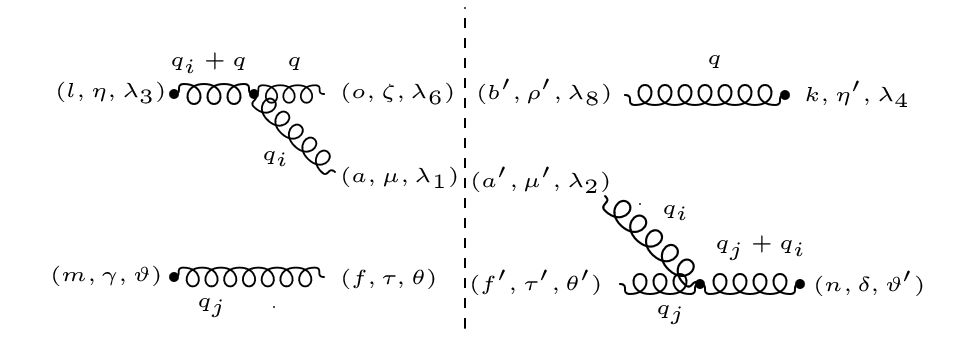
\includegraphics[width=0.95\textwidth]{images/GG/M1DaggerggInverse.png}
%\end{figure}
%
%
%\begin{equation}
%\begin{split}
%&M_1{M_2}^{\dagger}=\frac{g_s^2 f^{\:l\:o\:a} f^{\:f^{\prime}\: a^{\prime}\:n} \delta^{aa^{\prime}} \delta^{ob^{\prime}} \delta^{ff^{\prime}}}{(q_i +q)^2 (q_j +q_i)^2}
%[{g_{{\zeta}}}^{{\eta}^{\prime}} {g^{\gamma}}_{{\tau}^{\prime}}(g^{{\eta}{\zeta}}(2q+q_i)^{\mu}+g^{{\zeta}{\mu}}(q_i -q)^{\eta}-g^{{\mu}{\eta}}(2q_i +q)^{\zeta})\\
%&g_{{{\mu}}{{\mu}^{\prime}}}(g^{{{\tau}^{\prime}}{{\mu}^{\prime}}}(q_j-q_i)^{{\delta}}+g^{{{\mu}^{\prime}}{{\delta}}}(2q_i +q_j)^{{\tau}^{\prime}}-g^{{{\delta}}{{\tau}^{\prime}}}(2q_j+q_i)^{{\mu}^{\prime}}]
%\end{split}
%\end{equation}
%
%
%\begin{equation}
%\begin{split}
%&M_1{M_2}^{\dagger}=\frac{g_s^2 f^{\:l\:o\:a} f^{\:f\: a\:n}}{4(q\cdot q_i) (q_i \cdot q_j)}\\
%&[g^{{{\eta}}{{\eta}^{\prime}}}(2q+q_i)^{\gamma}(q_j-q_i)^{{\delta}}+g^{{{\eta}}{{\eta}^{\prime}}}(2q_i +q_j)^{\gamma}(2q+q_i)^{{\delta}}-g^{{{\eta}}{{\eta}^{\prime}}}g^{{{\gamma}}{{\delta}}}(2q+q_i)\cdot (2q_j+q_i)\\
%&+g^{{{\gamma}}{{\eta}^{\prime}}}(q_i -q)^{\eta}(q_j+q_i)^{{\delta}}+g^{{{\eta}^{\prime}}{{\delta}}}(q_i -q)^{\eta}(2q_i +q_j)^{{\gamma}}
%-g^{{{\gamma}}{{\delta}}}(q_i -q)^{\eta}(2q_j+q_i)^{{\eta}^{\prime}}\\
%&-g^{{{\gamma}}{{\eta}}}(2q_i +q)^{{\eta}^{\prime}}(q_j-q_i)^{{\delta}}
%-g^{{{\eta}}{{\delta}}}(2q_i +q)^{{\eta}^{\prime}}(2q_i +q_j)^{{\gamma}}
%+g^{{{\gamma}}{{\delta}}}(2q_j+q_i)^{{\eta}}(2q_i +q)^{{\eta}^{\prime}}]\\
%\end{split}
%\end{equation}
%
%\section{Parametrization in terms of $ (k_1 \cdot q_i )(q_i \cdot q_k) $}
%\begin{equation}
%	\begin{aligned}
%		\fbox{$  (k_1 \cdot q_i )(q_i \cdot q_k) {\color[RGB]{255,0,0} \: \approx\:} y\beta_1 (1-y)\:(p_i \cdot Q)(p_i \cdot p_k) $}
%    \end{aligned}
%\end{equation}
%
%\subsection*{Calculation of the third term}
%
%\begin{equation}
%\begin{split}
%&{\color[RGB]{255,0,0} -g^{{{\eta}}{{\eta}^{\prime}}}g^{{{\gamma}}{{\delta}}}}\lbrace 4{k_1}\cdot q_j+2k_1 \cdot q_i +2q_i \cdot q_k\rbrace
%\end{split}
%\end{equation}
%
%\begin{equation}
%\begin{split}
%&M_1{M_2}^{\dagger}=\frac{g_s^2 C_A}{4y\beta_1 (1-y)\:(p_i \cdot p_k)(p_i \cdot Q)}
%g^{{{\eta}}{{\eta}^{\prime}}}g^{{{\gamma}}{{\delta}}} \\
%&[4([\alpha_1 (1-y)+y\beta_1(\frac{Q^2}{2p_i \cdot Q})]\:p_i \cdot p_k+y\beta_1\:Q\cdot p_k+\sqrt{\alpha_1\beta_1y(1-y)} p_k \cdot {n_{\bot,1}})\\
%&2([\beta_1 (1-y)+y\alpha_1(\frac{Q^2}{2p_i \cdot Q})]\:p_i \cdot p_k+y\alpha_1\:Q\cdot p_k-\sqrt{\alpha_1\beta_1y(1-y)} p_k \cdot {n_{\bot,1}})\\
%&+2(y\:p_i\cdot Q)]\\
%\end{split}
%\end{equation}
%
%\begin{equation}
%\begin{split}
%&{\color[RGB]{255,0,0} -g^{{{\eta}}{{\eta}^{\prime}}}g^{{{\gamma}}{{\delta}}}}[ 4([\alpha_1 (1-y)+y\beta_1(\frac{Q^2}{2p_i \cdot Q})]\:p_i \cdot p_k+y\beta_1\:Q\cdot p_k+\sqrt{\alpha_1\beta_1y(1-y)} p_k \cdot {n_{\bot,1}})\\
%&2([\beta_1 (1-y)+y\alpha_1(\frac{Q^2}{2p_i \cdot Q})]\:p_i \cdot p_k+y\alpha_1\:Q\cdot p_k-\sqrt{\alpha_1\beta_1y(1-y)} p_k \cdot {n_{\bot,1}})\\
%&+2(y\:p_i\cdot Q)]
%\end{split}
%\end{equation}

\begin{equation}
\begin{split}
&{M_1{M_2}^{\dagger}}^{\prime}=g_s^2\: C_A\:g^{{{\eta}}{{\eta}^{\prime}}}g^{{{\gamma}}{{\delta}}}[\frac{1-\beta_1}{y\beta_1 (p_i \cdot Q)}+\frac{1}{2y(p_i \cdot Q)}+\frac{(1-\beta_1)(\frac{Q^2}{2p_i \cdot Q})}{2y\beta_1 (1-y)\:(p_i \cdot Q)}\\
&+\frac{(1-\beta_1)\:Q\cdot p_k}{2y\beta_1 (1-y)\:(p_i \cdot p_k)(p_i \cdot Q)}+\frac{1}{2(1-\beta_1)(1-y) (p_i \cdot p_k)}]\\
\end{split}
\end{equation}

\subsection{Summary of the results}

\begin{equation}
\begin{split}
&|M|^{2}=|{M^{\prime}}_2|^{2}+|{M^{\prime}}_1|^{2}+2RE(M_1{M_2}^{\dagger}+{M_1{M_2}^{\dagger}}^{\prime})\\
\end{split}
\end{equation}

\begin{equation}
\begin{split}
&{|{M}|}^2 =g_s^2\: C_A\:g^{{{\gamma}}{{\delta}}}[-2(1-\epsilon){\beta_1}(1-\beta_1){n^{{\eta}}}_{\bot,1}{n^{{\eta}^{\prime}}}_{\bot,1}+\frac{2\beta_1}{y(1-\beta_1) (p_i \cdot Q)}g^{{{\eta}}{{\eta}^{\prime}}}+\frac{2(1-\beta_1)}{y\beta_1 (p_i \cdot Q)}g^{{{\eta}}{{\eta}^{\prime}}}\\
&+\frac{Q^2}{2y\beta_1 (1-y)\:(p_i \cdot Q)(p_i \cdot Q)}g^{{{\eta}}{{\eta}^{\prime}}}+\frac{\:Q\cdot p_k}{y\beta_1 (1-y)\:(p_i \cdot p_k)(p_i \cdot Q)}g^{{{\eta}}{{\eta}^{\prime}}}]  \\
\end{split}
\end{equation}


Thus, the singular part from the matrix element after spin-averaging has full agreement with the splitting function $ \langle\:\hat{P_{gg}}\rangle\: $ from \ref{Alterali-Parisi}. This means that the desired result can be achieve by using the new kinematics in the collinear area.






















